\xchapter{Proposta}{}
\label{proposta}

Neste trabalho é proposto um módulo de identificação de momentos oportunos e inoportunos para interrupção de
motoristas, usando apenas sensores de smartphone. As seções estão estruturadas da seguinte forma: A seção
\ref{sec-arquitetura-solucao} apresenta a arquitetura da solução proposta. A seção \ref{sec-implementacao}
apresenta detalhes da implementação de cada módulo que compõe a solução.

\section{Arquitetura}
\label{sec-arquitetura-solucao}
Segundo \citeonline{garlan1993introduction}, a arquitetura de um software é a coleção de seus componentes computacionais - ou simplesmente
componentes - junto com a descrição das interações entre estes componentes - os conectores.  Sendo assim, nesta sessão
vamos mostrar os principais elementos da solução proposta e como eles interagem entre si.

O módulo funcionará em conjunto com o aplicativo Meu Possante, um aplicativo para sistemas Android e cuja arquitetura pode ser vista
na seção \ref{meupossante-app}. A identificação dos momentos oportunos e inoportunos é feita usando apenas sensores de smartphone,
sendo que os momentos oportunos são medidos utilizando o sensor de GPS, enquanto os inoportunos usam o giroscópio.

Os momentos escolhidos foram os seguintes:

\begin{itemize}
  \item Momentos Oportunos:
    \begin{itemize}
      \item Veículo parado \cite{kim2015sensors}
      \item Velocidade constante e menor que 29,5 km/h \cite{kim2015sensors}
    \end{itemize}
  \item Momentos Inoportunos:
    \begin{itemize}
      \item Durante uma curva \cite{monk2004recovering}
      \item Durante uma mudança de faixa \cite{monk2004recovering}
    \end{itemize}
\end{itemize}

O fluxo de dados da aplicação pode ser visto na figura x. O fluxo começa na coleta de dados do GPS e giroscópio, e termina
na decisão de notificação ou não do usuário. As setas na imagem representam o sentido do fluxo de dados.

\begin{figure}[h]
\centering
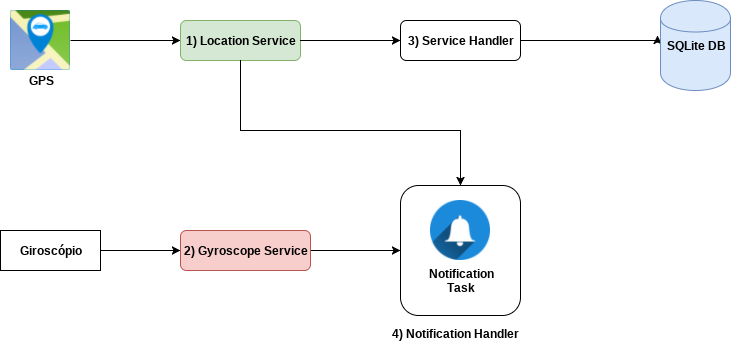
\includegraphics[width=0.7\textwidth]{images/arquitetura-meu-possante-com-modulo.png}
\caption{Arquitetura do Meu Possante após a implementação do módulo de identificação}
\label{arquitetura-meu-possante-com-modulo}
\end{figure}

Os módulos representados e suas funções são os seguintes:

\begin{enumerate}
  \item \textbf{Location Service:} Responsável pela coleta e monitoramento dos dados do GPS, incluindo deslocamento, velocidade e
  aceleração do dispositivo.
  \item \textbf{Gyroscope Service:} Responsável pela coleta e monitoramento dos dados do giroscópio. Este serviço detecta mudanças
  nos valores do sensor e aplica o algoritmo de detecção de curvas e mudanças de faixa.
  \item \textbf{Service Handler} Responsável pela inicialização e checagem de dados dos serviços
  que estão rodando na aplicação. Este módulo também é responsável por atualizar as informações
  de quilometragem no banco de dados e chamar o módulo de notificação quando necessário.
  \item \textbf{Notification Handler:} Responsável por consultar os serviços e decidir se deve criar uma notificação ou não naquele
  momento.
\end{enumerate}

Na próxima seção são dados mais detalhes sobre a implementação dos módulos, assim como os algoritmos utilizados.

\section{Implementação}
\label{sec-implementacao}

O projeto foi desenvolvido no Android Studio, o ambiente de desenvolvimento integrado (IDE) oficial para o
codificação de aplicativos Android. A linguagem utilizada foi o Java, linguagem padrão para o desenvolvimento
de aplicações Android.

As próximas subseções apresentam detalhes sobre a implementação de cada módulo que compõe a solução.

\subsection{Location Service}
\label{location-service}

O módulo \textit{Location Service} é o serviço responsável pela obtenção dos dados de GPS da aplicação. Os principais dados obtidos
por este serviço são a distância percorrida desde a última leitura, a velocidade e a aceleração.

Por ser necessário obter a localização do usuário em intervalos regulares, foi preciso especificar o intervalo de tempo em que a
aplicação iria requisitar atualizações da localização. Esta configuração tem impacto direto na autonomia de bateria do dispositivo,
pois quanto mais frequente é a requisição de dados do GPS, mais energia é gasta pelo dispositivo. O intervalo
de tempo escolhido foi de 5000ms (5 segundos), um intervalo razoavelmente frequente e que preserva a autonomia de bateria.
